\chapter{Nichtlineare Gleichungen}
Dies ist nötig beispielsweise in der Schaltungsanalyse inklusiver nichtlinearer Elemente (z.B. Diode, Transistor).

\begin{figure}
	\center
	\begin{circuitikz}
	\def\sourceX{0}
	\def\resistanceX{2}
	\def\diodeX{4}
	\def\upperY{4}
	\def\lowerY{0}
	
	\draw
		(\sourceX , \lowerY) to [I,i_=$I_0$] (\sourceX , \upperY)
		(\resistanceX , \lowerY) to [R=$R_0$,*-*,v=$u$] (\resistanceX , \upperY)
		(\sourceX , \upperY) to (\resistanceX , \upperY)
		(\sourceX , \lowerY) to (\resistanceX , \lowerY)
	;
	
	\draw
		(\diodeX , \upperY) to [D,v_>=$u_d$,i=$i_d$] (\diodeX, \lowerY)	
		(\resistanceX , \upperY) to (\diodeX , \upperY)
		(\resistanceX , \lowerY) to (\diodeX , \lowerY)
	;
\end{circuitikz} 

	\caption{Beispiel einer Schaltung}
\end{figure}

Gesucht sei hierbei das stationäre Verhalten bei konstanter Erregung (\emph{DC-Arbeitspunkt}). Die Diode kann mithilfe von $i_D = I_S \cdot \left(e^{\frac{u_D}{U_T}} - 1\right)$ beschrieben werden. Daraus folgt dann
\[I_0 - \frac{u_D}{R} = I_S \cdot \left(e^{\frac{u_D}{U_T}} - 1\right)\]
Gesucht ist somit die Nullstelle von
\[F(u_D) = f(u_D) - g(u_D) = 0\]
Nullstellensuchen sind meist iterative Verfahren welche aus einem Startwert $\vec{x}$ eine Lösung $\vec{x}^\star$ mit $F(\vec{x}^\star) = 0$ ermitteln. Zuerst einmal wollen wir das Problem eindimensional betrachten:
\[F(x) = 0\]
Gegeben ist dabei ein $F(x)$, welches stetig auf $[a, b]$ ist mit $F(a) \cdot F(b) < 0$ und gesucht ist $x^\star$ mit $F(x^\star) = 0$, $a \le x^\star \le b$.

\begin{figure}
	\center
	\begin{tikzpicture}
	\draw[thick,->] (0,0) -- (4,0) node[right]{$u_D$};
	\draw[thick,->] (0,0) -- (0,3) node[above]{$i_D$};
	
	\draw[blue,domain=0:2,name path=exp] plot (\x,{exp(0.7*\x)-1});
	\draw[red,domain=0:3,name path=line] (0,2) node [left] {$I_0$} -- (3,0) node [below] {$I_0 R_0$};
	\path [name intersections={of=exp and line,by=intersect}];
	
	\filldraw [color=red] (intersect) circle (2pt);
	\draw (intersect) node [right=0.2] {Lösungspunkt};
	\draw [dashed] (intersect) -- ($(0,0)!(intersect)!(4,0)$) node [below] {$U_D^*$};
	
	\begin{scope}[shift={(6,1.5)}]
		\draw[thick,->, name path=xaxis] (-0.1,0) -- (4,0) node[right]{$u_D$};
		\draw[thick,->] (0,-3) -- (0,3) node[above]{$F(u_D)$};
		
		\draw[domain=0:2.5,name path=exp] plot (\x,{exp(0.7*\x)-3}) node [right] {$F(u_D)$};
		
		\path [name intersections={of=exp and xaxis,by=intersect}];
		\draw [<-, thick, >=stealth] (intersect)  -- ++(0.5,0.5) node [right] {Lösungspunkt};
		\draw (0,-2)node [left] {$-I_0$};		
	\end{scope}	
\end{tikzpicture} 

	\caption{Arbeitspunktermittlung durch Nullstellensuche}
\end{figure}

\section{Intervallhalbierung}
\begin{enumerate}
	\item Startintervall $[a^{(0)}, b^{(0)}] = [a, b]$, $k = 0$
	\item Intervallmitte $m = \frac{a^{(k)} + b^{(k)}}{2}$
	\item $[a^{k + 1)}, b^{(k + 1)}] = \begin{cases} [m, b^{(k)}] & \text{fuer\ } F(m) \cdot F(a^{(k)}) > 0 \\ [a^{(k)}, m] & \text{fuer\ } F(m) \cdot F(a^{(k)}) < 0 \end{cases}$
	\item Falls $\abs{a^{(k + 1)} - b^{k + 1)}} > \epsilon$ dann gehe zu Schritt 2, $k = k + 1$
\end{enumerate}

\begin{figure}
	\center
	\begin{tikzpicture}
	\coordinate (a) at (0,0);
	\coordinate (b) at (5,0);
	
	\draw [thick] (a) node [left] {$a$} -- (b) node[right] {$b$};
	\draw[thick] (a) -- ++(0,-1) node[left] {$f(a)$} [out=10,in=-115] to (1.5625,0) node[above] {\color{red}{$\xi$}} [out=65,in=185] to (5,3);
	\draw[thick] (b) -- ++(0,3) node[right] {$f(b)$};
	
	\draw[thick,dashed] ($(a)!.25!(b)$) -- ++(0,-.45);
	\draw[thick,dashed] ($(a)!.375!(b)$) -- ++(0,.6);
	\draw[thick,dashed] ($(a)!.5!(b)$) -- ++(0,1.6);
	
	\draw[thick] (0,-2) node [left] {$a_0$} -- (5,-2) node[right] {$b_0$};
	\draw[thick] (0,-1.9) -- (0,-2.1); 
	\draw[thick] (5,-1.9) -- (5,-2.1);
	\draw[thick] (2.5,-1.9) node[above] {\color{red}{$x_1$}} -- (2.5,-2.1); 
	\draw[thick] (0,-3) node [left] {$a_1$} -- (2.5,-3) node[right] {$b_1$};
	\draw[thick] (0,-2.9) -- (0,-3.1); 
	\draw[thick] (2.5,-2.9) -- (2.5,-3.1);
	\draw[thick] (1.25,-2.9) node[above] {\color{red}{$x_2$}} -- (1.25,-3.1);
	\draw[thick] (1.25,-4) node [left] {$a_2$} -- (2.5,-4) node[right] {$b_2$};
	\draw[thick] (1.25,-3.9) -- (1.25,-4.1); 
	\draw[thick] (2.5,-3.9) -- (2.5,-4.1);
	\draw[thick] (1.875,-3.9) node[above] {\color{red}{$x_3$}} -- (1.875,-4.1);
	\draw[thick] (1.25,-5) node [left] {$a_3$} -- (1.875,-5) node[right] {$b_3$};
	\draw[thick] (1.25,-4.9) -- (1.25,-5.1); 
	\draw[thick] (1.875,-4.9) -- (1.875,-5.1); 
\end{tikzpicture} 

	\caption{Intervallhalbierung}
\end{figure}

Die Konvergenz eines iterativen Verfahrens wird mithilfe der Parameter $L$, dem Konvergenzfaktor, und $p$, der Konvergenzordnung, beschrieben.
\[\Delta^{(k + 1)} = \frac{1}{2} \Delta^{(k)} = (\frac{1}{2})^{k + 1} \Delta^{(0)}\]
\[\epsilon = x - x^\star\]
\[\abs{\epsilon^{(k + 1)}} \le L \abs{\epsilon^{(k)}}^p\]
Die Intervallhalbierung liegt bei $p = 1$, also linearer Konvergenz, und $L = 1/2$. Die Anzahl der Iterationsschritte bis zu einem Restfehler $\Delta^R$ ist damit
\[\kappa = \ceil{\log2 \left( \frac{\Delta^{(0)}}{\Delta^R}\right)}\]

\begin{figure}
	\center
	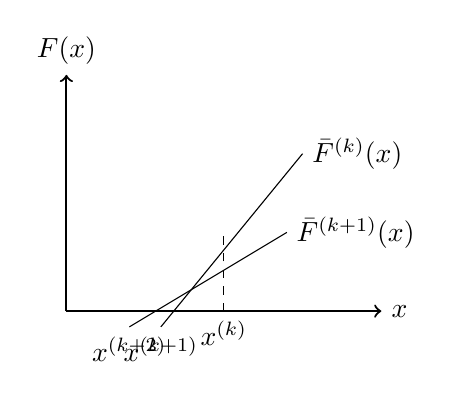
\begin{tikzpicture}
	\draw[thick,->] (0,0) -- (4,0) node[right]{$x$};
	\draw[thick,->] (0,0) -- (0,3) node[above]{$F(x)$};
	
	\draw (0.8, -0.2) node [below] {$x^{(k+2)}$} -- (2.8, 1) node [right] {$\bar{F}^{(k+1)}(x)$};
	\draw (1.2, -0.2) node [below] {$x^{(k+1)}$} -- (3, 2) node [right] {$\bar{F}^{(k)}(x)$};
	
	\draw [dashed] (2, 0) node [below] {$x^{(k)}$} -- ++(0,1);	
\end{tikzpicture} 

	\caption{Newton-Iteration}
\end{figure}

\section{Newton-Raphson-Verfahren} Die Idee hinter dem Newton-Raphson-Verfahren ist eine Taylorreihe erster Ordnung:
\[F(x) = F(x^{(k)}) + F'(x^{(k)}) \cdot (x - x^{(k)}) + F''(x^{(k)}) \cdot \frac{(x - x^{(k)})^2}{2} + \dots\]
\[x^{(k + 1)} = x^{(k)} - \frac{F(x^{(k)})}{F'(x^{(k)})}\]

Das Konvergenzverhalten des Newton-Raphson-Verfahrens erhält man aus einer Taylorreihe:
\[x^{(k + 1)} = x^{(k)} - \frac{F(x^\star) + F'(x^\star)(x^{(k)} - x^\star) + \frac{1}{2} F''(x^\star) \cdot {\epsilon^{k}}^2 + ... + \frac{1}{n!} F^{(n)}(x^\star) \cdot {\epsilon^{k}}^n}{F'(x^\star) + F''(x^\star) \cdot \epsilon^{(k)} + \frac{1}{(n - 1)!} \cdot F^{(n)} {\epsilon^{(k)}}^{n - 1}}\]
\[\epsilon^{(k + 1)} = \epsilon^{(k)} \left( 1 - \frac{F' + \frac{1}{2} F'' \cdot \epsilon^{(k)} + \dots}{F' + F'' \cdot \epsilon^{(k)} + \dots} \right) \approx \epsilon^{(k)} \left( \left(1 + \frac{1}{2} \epsilon^{(k)} \frac{F''}{F'} \right) \cdot \left( 1 - \frac{1}{2} \epsilon^{(k)} \frac{F''}{F'} \right) \right)\]
\[\epsilon^{(k + 1)} \approx \epsilon^{(k)} \left( 1 - \left( 1 + \frac{1}{2} \cdot \epsilon^{(k)} \frac{F''}{F'} - \epsilon^{(k)} \frac{F''}{F'}\right)\right) = \frac{1}{2} \cdot {\epsilon^{(k)}}^2 \frac{F''}{F'}\]

Probleme beim Newton-Raphson-Verfahren treten bei n-fachen Nullstellen ($F'(x^\star) = \dots = F^{(n - 1)}(x^\star) = 0)$, $F^{(n)}(x^\star) \ne 0$) auf.
\[\epsilon^{(k + 1)} \approx \epsilon^{(k)} \cdot \left( 1 - \frac{(n - 1)!}{n!}\right) - \epsilon^{(k)} \cdot \left( 1 - \frac{1}{n}\right) = \epsilon^{(k)} \frac{n - 1}{n}\]
Somit erhält man nur mehr lineare Konvergenz.
z.B.: $F(x) = e^x - 1 \Rightarrow x^{(k + 1)} = x^{(k)} - \frac{e^{x^{(k)}} - 1}{e^{x^{(k)}}}$

\subsection{Variation: Sekanten-Methode}
\[F'(x^{(k)}) = \lim_{x \rightarrow x^{(k)}} \frac{F(x) - F(x^{(k)})}{x - x^{(k)}}\]
\[F'(x^{(k)}) = \frac{F(x^{(k - 1)}) - F(x^{(k)})}{x^{(k - 1)} - x^{(k)}}\]
Eingesetzt in die Newton-Gleichung erhält man somit
\[x^{(k + 1)} = x^{(k)} - \frac{F(x^{(k)}) \cdot (x^{(k)} - x^{(k - 1)})}{F(x^{(k)}) - F(x^{(k - 1)})}\]
Dadurch ist pro Schritt nur eine Funktionsauswertung nötig.

\section{Fixpunktiteration}
Fixpunkt $x^*$ einer Funktion $g(x)$
\begin{equation}
	x^* = g(x^*)
\end{equation}
Nullstellenproblem und Fixpunktproblem können ineinander überführt werden., z.B.
\[g(x) = x - F(x)\]

\subsection{Fixpunkttheorem}
\begin{enumerate}
	\item Sei $g(x)$ stetig auf $[a,b]$, sowie $g(x)\in [a,b]$ für alle $x\in [a,b]$.\\
	Dann hat $g(x)$ mindestens einen Fixpunkt auf $[a,b]$
	\item Existiere zusätzlich $g'(x)$ auf $(a,b)$, sowie eine positive Konstante $k<1$ mit \mbox{$\abs{g'(x)}\leq k$}, für alle $x\in (a,b)$
	\begin{itemize}
		\item Dann hat $g(x)$ exakt einen Fixpunkt auf $[a,b]$
		\item Gilt $0<k<1$, dann konvergiert für jedes $x^{(0)}\in [a,b]$ die Folge
		\[x^{(n)} = g(x^{(n-1)})\quad,n\geq 1\]
		zum eindeutigen Fixpunkt $x^*\in [0,b]$.
	\end{itemize}
\end{enumerate}

\subsection{Konvergenzverhalten iterativer Verfahren}
\begin{align}
	x^{(k+1)} &= g(x^{(k)}) & \text{Iterationsvorschrift}\\
	x^* &= g(x^*) & \text{Fixpunkt}
\end{align}

Taylorreihe von $g(x)$ um $x^*$
\begin{align}
	\left[g(x^{(k)})\right]x^{(k+1)} &= \underbrace{g(x^*)}_{x^*} + g'(x^*)\cdot (x^{(k)}-x^*) + \frac{1}{2} g''(x^*)\cdot (x^{(k)}-x^*)^2 + \ldots\\
	\varepsilon^{(k+1)} &= g'(x^*)\cdot \varepsilon^{(k)} + \frac{1}{2} g''(x^*)\cdot {\varepsilon^{(k)}}^2 + \ldots
\end{align}
\begin{itemize}
	\item $g'(x^*)\neq 0$, $\abs{g'(x^*)} < 1 \quad\rightarrow$ lineare Konvergenz
	\item $g'(x^*) = 0$, $g''(x^*)\neq 0 \quad\Rightarrow$ quadratische Konvergenz ("Konstruktionshinweis")
\end{itemize}

\begin{figure}
	\center
	\begin{tikzpicture}
	\draw[thick,->] (0,0) -- (4,0) node[right]{$x^{(i)}$};
	\draw[thick,->] (0,0) -- (0,4) node[above]{$x^{(i + 1)} = g(x^{(i)})$};
	
	\draw (0, -0) node [below] {$x^{(k+2)}$} -- (4, 4);
	\draw[blue,domain=0:4,name path=exp] plot (\x,{exp(0.3*\x)});
	
	\def\xZero{3.5}
	\def\xOne{2.85765111806316378986}
	\def\xTwo{2.35677777239982118523}
	\def\xThree{2.02796602315439250323}
	\def\xFour{1.83747033351067410687}
			
	\draw [dashed,gray] (\xZero, 0) node [below,black] {$x^{(0)}$} -- (\xZero, \xOne);
	\draw [dashed,gray] (0, \xOne) node [left,black] {$g(x^{(0)})$} -- (\xZero, \xOne);
	
	\draw [dashed,gray] (\xOne, 0) node [above,black] {$x^{(1)}$} -- (\xOne, \xTwo);
	\draw [dashed,gray] (0, \xTwo) node [right,black] {$g(x^{(1)})$} -- (\xOne, \xTwo);
	
	\draw [dashed,gray] (\xTwo, 0) node [below,black] {$x^{(2)}$} -- (\xTwo, \xThree);
	\draw [dashed,gray] (0, \xThree) node [left,black] {$g(x^{(2)})$} -- (\xTwo, \xThree);
	
	\draw [dashed,gray] (\xThree, 0) node [above,black] {$x^{(3)}$} -- (\xThree, \xFour);
	\draw [dashed,gray] (0, \xFour) node [right,black] {$g(x^{(3)})$} -- (\xThree, \xFour);
\end{tikzpicture} 

	\caption{Fixpunktiteration}
\end{figure}

\section{Mehrdimensionales Newton-Raphson-Verfahren}
\begin{align}
	\vec{F}(\vec{x}) &= \vec{0}\quad,\vec{F} = (F_1,\ldots,F_r)^T\\
	\vec{F}(\vec{x}^{(k+1)}) &= \vec{F}(\vec{x}^{(k)}) + \underbrace{\frac{\partial\vec{F}(\vec{x}^{(k)})}{\partial\vec{x}^T}} \cdot\left(\vec{x}^{(k+1)}-\vec{x}^{(k)}\right)\\
	\begin{matrix}
	\text{Jacobi-Matrix}\\ \text{Fundamentalmatrix}
	\end{matrix}\qquad & \ma{J}(\vec{x}) = \frac{\partial\vec{F}(\vec{x})}{\partial\vec{x}^T} = \left(\frac{\partial\vec{F}}{\partial\vec{x}_1},\ldots,\frac{\partial\vec{F}}{\partial\vec{x}_r}\right) =\begin{pmatrix}
	\frac{\partial\vec{F}_1}{\partial\vec{x}_1} & \ldots & \frac{\partial\vec{F}_1}{\partial\vec{x}_r}\\
	\vdots & & \vdots\\
	\frac{\partial\vec{F}_r}{\partial\vec{x}_1} & \ldots & \frac{\partial\vec{F}_r}{\partial\vec{x}_r}
	\end{pmatrix}\\
	\vec{F}(\vec{x}^{(k+1)}) &= \vec{0}\Rightarrow\ma{J}(\vec{x}^{(k)})\cdot\left(\vec{x}^{(k+1)}-\vec{x}^{(k)}\right) = -\vec{F}(\vec{x}^{(k)})
\end{align}
\[\vec{x}^{(k+1)} = \vec{x}^{(k)}-\ma{J}^{-1}(\vec{x}^{(k)})\cdot\vec{F}(\vec{x}^{(k)})\]
\textbf{Praktisch:}
\[\ma{J}(\vec{x}^{(k)})\cdot\vec{x}^{(k+1)} = \ma{J}(\vec{x}^{(k)})\cdot\vec{x}^{(k)} - \vec{F}(\vec{x}^{(k)})\]

\subsection{Konvergenz}
\[\vec x^{(k + 1)} = \vec \Phi(\vec x^{(k)}) = \vec \Phi(\vec x^\star) + \frac{\partial \vec \Phi}{\partial \vec x^T} \bigg|_{\vec x  = \vec x^\star} \cdot \left( \vec x^{(k)} - \vec x^\star \right) + \mathcal O\left( \left( \vec x^{(k)} - \vec x^\star \right) \cdot \left( \vec x^{(k)} - \vec x^\star \right)^T\right)\]

\[\vec \epsilon^{(k + 1)} = \frac{\partial \vec \Phi}{\partial \vec x^T} \bigg|_{\vec x = \vec x^\star} \vec \epsilon^{(k)} + \mathcal O \left( \vec \epsilon^{(k)} \cdot \vec \epsilon^{{(k)}^T} \right)\]

\[\vec \Phi(\vec x) = \vec x - \ma{J}^{-1} \cdot \vec F\]
\[\frac{\partial \vec \Phi}{\partial \vec x^T} = \underbrace{\ma{E} - \underbrace{\ma{J}^{-1} \underbrace{\frac{\partial \vec F}{\partial \vec x^T}}_{\ma J^{-1}}}_{\ma E}}_{\ma 0} - \underbrace{\frac{\partial \ma{J}^{-1}}{\partial \vec x^T} \cdot \vec F}_{\ma 0}\]

\subsection{Abbruchkriterien}
Gegeben sei eine Nullstellen-Suche: $\vec F(\vec x) = \vec 0 \Rightarrow \vec x^\star$

Als Abbruchkriterium wäre schön
\[||\vec x^{(k)} - \vec x^\star|| = || \vec \epsilon^{(k)} || \le || \vec \epsilon^{(A)} ||\]
oder
\[\frac{|| \vec \epsilon^{(k)} ||}{|| \vec x^\star ||} \le || \vec \epsilon^{(R)} ||\]
Problematisch dabei ist, dass $\vec x^\star$ unbekannt ist. Daher muss man in der Anwendung ein anderes Kriterium wählen:
\begin{itemize}
	\item $||\vec x^{(k + 1)} - \vec x^{(k)} || \le || \vec \epsilon^{(A)} ||$ bzw. $\frac{||\vec x^{(k + 1)} - \vec x^{(k)}||}{|| \vec x^{(k + 1)} ||} \le || \vec \epsilon^{(R)} ||$
	\item $||\vec F(\vec x^{(k + 1)}) - \vec F(\vec x^{(k)})|| \le \Delta_F^{(A)}$
	\item $||\vec F(\vec x^{(k)})|| \le F_{min}$
	\item $k > k_{max}$
\end{itemize}
